
%% bare_conf.tex
%% V1.3
%% 2007/01/11
%% by Michael Shell
%% See:
%% http://www.michaelshell.org/
%% for current contact information.
%%
%% This is a skeleton file demonstrating the use of IEEEtran.cls
%% (requires IEEEtran.cls version 1.7 or later) with an IEEE conference paper.
%%
%% Support sites:
%% http://www.michaelshell.org/tex/ieeetran/
%% http://www.ctan.org/tex-archive/macros/latex/contrib/IEEEtran/
%% and
%% http://www.ieee.org/

%%*************************************************************************
%% Legal Notice:
%% This code is offered as-is without any warranty either expressed or
%% implied; without even the implied warranty of MERCHANTABILITY or
%% FITNESS FOR A PARTICULAR PURPOSE! 
%% User assumes all risk.
%% In no event shall IEEE or any contributor to this code be liable for
%% any damages or losses, including, but not limited to, incidental,
%% consequential, or any other damages, resulting from the use or misuse
%% of any information contained here.
%%
%% All comments are the opinions of their respective authors and are not
%% necessarily endorsed by the IEEE.
%%
%% This work is distributed under the LaTeX Project Public License (LPPL)
%% ( http://www.latex-project.org/ ) version 1.3, and may be freely used,
%% distributed and modified. A copy of the LPPL, version 1.3, is included
%% in the base LaTeX documentation of all distributions of LaTeX released
%% 2003/12/01 or later.
%% Retain all contribution notices and credits.
%% ** Modified files should be clearly indicated as such, including  **
%% ** renaming them and changing author support contact information. **
%%
%% File list of work: IEEEtran.cls, IEEEtran_HOWTO.pdf, bare_adv.tex,
%%                    bare_conf.tex, bare_jrnl.tex, bare_jrnl_compsoc.tex
%%*************************************************************************

% *** Authors should verify (and, if needed, correct) their LaTeX system  ***
% *** with the testflow diagnostic prior to trusting their LaTeX platform ***
% *** with production work. IEEE's font choices can trigger bugs that do  ***
% *** not appear when using other class files.                            ***
% The testflow support page is at:
% http://www.michaelshell.org/tex/testflow/



% Note that the a4paper option is mainly intended so that authors in
% countries using A4 can easily print to A4 and see how their papers will
% look in print - the typesetting of the document will not typically be
% affected with changes in paper size (but the bottom and side margins will).
% Use the testflow package mentioned above to verify correct handling of
% both paper sizes by the user's LaTeX system.
%
% Also note that the "draftcls" or "draftclsnofoot", not "draft", option
% should be used if it is desired that the figures are to be displayed in
% draft mode.
%
\documentclass[10pt, conference, compsocconf]{IEEEtran}
% Add the compsocconf option for Computer Society conferences.
%
% If IEEEtran.cls has not been installed into the LaTeX system files,
% manually specify the path to it like:
% \documentclass[conference]{../sty/IEEEtran}





% Some very useful LaTeX packages include:
% (uncomment the ones you want to load)


% *** MISC UTILITY PACKAGES ***
%
%\usepackage{ifpdf}
% Heiko Oberdiek's ifpdf.sty is very useful if you need conditional
% compilation based on whether the output is pdf or dvi.
% usage:
% \ifpdf
%   % pdf code
% \else
%   % dvi code
% \fi
% The latest version of ifpdf.sty can be obtained from:
% http://www.ctan.org/tex-archive/macros/latex/contrib/oberdiek/
% Also, note that IEEEtran.cls V1.7 and later provides a builtin
% \ifCLASSINFOpdf conditional that works the same way.
% When switching from latex to pdflatex and vice-versa, the compiler may
% have to be run twice to clear warning/error messages.






% *** CITATION PACKAGES ***
%
\usepackage{cite}
% cite.sty was written by Donald Arseneau
% V1.6 and later of IEEEtran pre-defines the format of the cite.sty package
% \cite{} output to follow that of IEEE. Loading the cite package will
% result in citation numbers being automatically sorted and properly
% "compressed/ranged". e.g., [1], [9], [2], [7], [5], [6] without using
% cite.sty will become [1], [2], [5]--[7], [9] using cite.sty. cite.sty's
% \cite will automatically add leading space, if needed. Use cite.sty's
% noadjust option (cite.sty V3.8 and later) if you want to turn this off.
% cite.sty is already installed on most LaTeX systems. Be sure and use
% version 4.0 (2003-05-27) and later if using hyperref.sty. cite.sty does
% not currently provide for hyperlinked citations.
% The latest version can be obtained at:
% http://www.ctan.org/tex-archive/macros/latex/contrib/cite/
% The documentation is contained in the cite.sty file itself.






% *** GRAPHICS RELATED PACKAGES ***
%
\ifCLASSINFOpdf
  \usepackage[pdftex]{graphicx}
  % declare the path(s) where your graphic files are
  \graphicspath{{../pdf/}{./figures/}}
  % and their extensions so you won't have to specify these with
  % every instance of \includegraphics
  \DeclareGraphicsExtensions{.pdf,.jpeg,.png}
\else
  % or other class option (dvipsone, dvipdf, if not using dvips). graphicx
  % will default to the driver specified in the system graphics.cfg if no
  % driver is specified.
  % \usepackage[dvips]{graphicx}
  % declare the path(s) where your graphic files are
  % \graphicspath{{../eps/}}
  % and their extensions so you won't have to specify these with
  % every instance of \includegraphics
  % \DeclareGraphicsExtensions{.eps}
\fi
% graphicx was written by David Carlisle and Sebastian Rahtz. It is
% required if you want graphics, photos, etc. graphicx.sty is already
% installed on most LaTeX systems. The latest version and documentation can
% be obtained at: 
% http://www.ctan.org/tex-archive/macros/latex/required/graphics/
% Another good source of documentation is "Using Imported Graphics in
% LaTeX2e" by Keith Reckdahl which can be found as epslatex.ps or
% epslatex.pdf at: http://www.ctan.org/tex-archive/info/
%
% latex, and pdflatex in dvi mode, support graphics in encapsulated
% postscript (.eps) format. pdflatex in pdf mode supports graphics
% in .pdf, .jpeg, .png and .mps (metapost) formats. Users should ensure
% that all non-photo figures use a vector format (.eps, .pdf, .mps) and
% not a bitmapped formats (.jpeg, .png). IEEE frowns on bitmapped formats
% which can result in "jaggedy"/blurry rendering of lines and letters as
% well as large increases in file sizes.
%
% You can find documentation about the pdfTeX application at:
% http://www.tug.org/applications/pdftex





% *** MATH PACKAGES ***
%
\usepackage[cmex10]{amsmath}
% A popular package from the American Mathematical Society that provides
% many useful and powerful commands for dealing with mathematics. If using
% it, be sure to load this package with the cmex10 option to ensure that
% only type 1 fonts will utilized at all point sizes. Without this option,
% it is possible that some math symbols, particularly those within
% footnotes, will be rendered in bitmap form which will result in a
% document that can not be IEEE Xplore compliant!
%
% Also, note that the amsmath package sets \interdisplaylinepenalty to 10000
% thus preventing page breaks from occurring within multiline equations. Use:
%\interdisplaylinepenalty=2500
% after loading amsmath to restore such page breaks as IEEEtran.cls normally
% does. amsmath.sty is already installed on most LaTeX systems. The latest
% version and documentation can be obtained at:
% http://www.ctan.org/tex-archive/macros/latex/required/amslatex/math/





% *** SPECIALIZED LIST PACKAGES ***
%
\usepackage{algorithm}
\usepackage{algorithmic}
% algorithmic.sty was written by Peter Williams and Rogerio Brito.
% This package provides an algorithmic environment fo describing algorithms.
% You can use the algorithmic environment in-text or within a figure
% environment to provide for a floating algorithm. Do NOT use the algorithm
% floating environment provided by algorithm.sty (by the same authors) or
% algorithm2e.sty (by Christophe Fiorio) as IEEE does not use dedicated
% algorithm float types and packages that provide these will not provide
% correct IEEE style captions. The latest version and documentation of
% algorithmic.sty can be obtained at:
% http://www.ctan.org/tex-archive/macros/latex/contrib/algorithms/
% There is also a support site at:
% http://algorithms.berlios.de/index.html
% Also of interest may be the (relatively newer and more customizable)
% algorithmicx.sty package by Szasz Janos:
% http://www.ctan.org/tex-archive/macros/latex/contrib/algorithmicx/




% *** ALIGNMENT PACKAGES ***
%
%\usepackage{array}
% Frank Mittelbach's and David Carlisle's array.sty patches and improves
% the standard LaTeX2e array and tabular environments to provide better
% appearance and additional user controls. As the default LaTeX2e table
% generation code is lacking to the point of almost being broken with
% respect to the quality of the end results, all users are strongly
% advised to use an enhanced (at the very least that provided by array.sty)
% set of table tools. array.sty is already installed on most systems. The
% latest version and documentation can be obtained at:
% http://www.ctan.org/tex-archive/macros/latex/required/tools/


%\usepackage{mdwmath}
%\usepackage{mdwtab}
% Also highly recommended is Mark Wooding's extremely powerful MDW tools,
% especially mdwmath.sty and mdwtab.sty which are used to format equations
% and tables, respectively. The MDWtools set is already installed on most
% LaTeX systems. The lastest version and documentation is available at:
% http://www.ctan.org/tex-archive/macros/latex/contrib/mdwtools/


% IEEEtran contains the IEEEeqnarray family of commands that can be used to
% generate multiline equations as well as matrices, tables, etc., of high
% quality.


%\usepackage{eqparbox}
% Also of notable interest is Scott Pakin's eqparbox package for creating
% (automatically sized) equal width boxes - aka "natural width parboxes".
% Available at:
% http://www.ctan.org/tex-archive/macros/latex/contrib/eqparbox/





% *** SUBFIGURE PACKAGES ***
\usepackage[tight,footnotesize]{subfigure}
% subfigure.sty was written by Steven Douglas Cochran. This package makes it
% easy to put subfigures in your figures. e.g., "Figure 1a and 1b". For IEEE
% work, it is a good idea to load it with the tight package option to reduce
% the amount of white space around the subfigures. subfigure.sty is already
% installed on most LaTeX systems. The latest version and documentation can
% be obtained at:
% http://www.ctan.org/tex-archive/obsolete/macros/latex/contrib/subfigure/
% subfigure.sty has been superceeded by subfig.sty.



%\usepackage[caption=false]{caption}
%\usepackage[font=footnotesize]{subfig}
% subfig.sty, also written by Steven Douglas Cochran, is the modern
% replacement for subfigure.sty. However, subfig.sty requires and
% automatically loads Axel Sommerfeldt's caption.sty which will override
% IEEEtran.cls handling of captions and this will result in nonIEEE style
% figure/table captions. To prevent this problem, be sure and preload
% caption.sty with its "caption=false" package option. This is will preserve
% IEEEtran.cls handing of captions. Version 1.3 (2005/06/28) and later 
% (recommended due to many improvements over 1.2) of subfig.sty supports
% the caption=false option directly:
%\usepackage[caption=false,font=footnotesize]{subfig}
%
% The latest version and documentation can be obtained at:
% http://www.ctan.org/tex-archive/macros/latex/contrib/subfig/
% The latest version and documentation of caption.sty can be obtained at:
% http://www.ctan.org/tex-archive/macros/latex/contrib/caption/




% *** FLOAT PACKAGES ***
%
%\usepackage{fixltx2e}
% fixltx2e, the successor to the earlier fix2col.sty, was written by
% Frank Mittelbach and David Carlisle. This package corrects a few problems
% in the LaTeX2e kernel, the most notable of which is that in current
% LaTeX2e releases, the ordering of single and double column floats is not
% guaranteed to be preserved. Thus, an unpatched LaTeX2e can allow a
% single column figure to be placed prior to an earlier double column
% figure. The latest version and documentation can be found at:
% http://www.ctan.org/tex-archive/macros/latex/base/



%\usepackage{stfloats}
% stfloats.sty was written by Sigitas Tolusis. This package gives LaTeX2e
% the ability to do double column floats at the bottom of the page as well
% as the top. (e.g., "\begin{figure*}[!b]" is not normally possible in
% LaTeX2e). It also provides a command:
%\fnbelowfloat
% to enable the placement of footnotes below bottom floats (the standard
% LaTeX2e kernel puts them above bottom floats). This is an invasive package
% which rewrites many portions of the LaTeX2e float routines. It may not work
% with other packages that modify the LaTeX2e float routines. The latest
% version and documentation can be obtained at:
% http://www.ctan.org/tex-archive/macros/latex/contrib/sttools/
% Documentation is contained in the stfloats.sty comments as well as in the
% presfull.pdf file. Do not use the stfloats baselinefloat ability as IEEE
% does not allow \baselineskip to stretch. Authors submitting work to the
% IEEE should note that IEEE rarely uses double column equations and
% that authors should try to avoid such use. Do not be tempted to use the
% cuted.sty or midfloat.sty packages (also by Sigitas Tolusis) as IEEE does
% not format its papers in such ways.





% *** PDF, URL AND HYPERLINK PACKAGES ***
%
%\usepackage{url}
% url.sty was written by Donald Arseneau. It provides better support for
% handling and breaking URLs. url.sty is already installed on most LaTeX
% systems. The latest version can be obtained at:
% http://www.ctan.org/tex-archive/macros/latex/contrib/misc/
% Read the url.sty source comments for usage information. Basically,
% \url{my_url_here}.


\usepackage{amsthm}

\theoremstyle{plain}
\newtheorem{thm}{Theorem} % reset theorem numbering for each chapter
\theoremstyle{definition}
\newtheorem{defn}[thm]{Definition} % definition numbers are dependent on theorem numbers
\newtheorem{exmp}[thm]{Example} 

% *** Do not adjust lengths that control margins, column widths, etc. ***
% *** Do not use packages that alter fonts (such as pslatex).         ***
% There should be no need to do such things with IEEEtran.cls V1.6 and later.
% (Unless specifically asked to do so by the journal or conference you plan
% to submit to, of course. )


% correct bad hyphenation here
\hyphenation{op-tical net-works semi-conduc-tor}


\begin{document}
%
% paper title
% can use linebreaks \\ within to get better formatting as desired
\title{An Intelligent Middleware Support for Service-Oriented IoT Systems}


% author names and affiliations
% use a multiple column layout for up to two different
% affiliations

\author{
\IEEEauthorblockN{Shih-Yuan Yu, Chi-Sheng Shih, Jane Yung-jen Hsu}
\IEEEauthorblockA{Dept of Computer Science and Information Engineering, \\
National Taiwan University\\
Taipei, Taiwan\\
r01922040@ntu.edu.tw, cshih@csie.ntu.edu.tw, \\ yjhsu@csie.ntu.edu.tw}
\and
\IEEEauthorblockN{Kwei Jay Lin}
\IEEEauthorblockA{Dept of Electrical Engineering and Computer Science\\
University of California, Irvine\\
Irvine, California, USA\\
klin@uci.edu}
}

% conference papers do not typically use \thanks and this command
% is locked out in conference mode. If really needed, such as for
% the acknowledgment of grants, issue a \IEEEoverridecommandlockouts
% after \documentclass

% for over three affiliations, or if they all won't fit within the width
% of the page, use this alternative format:
% 
%\author{\IEEEauthorblockN{Michael Shell\IEEEauthorrefmark{1},
%Homer Simpson\IEEEauthorrefmark{2},
%James Kirk\IEEEauthorrefmark{3}, 
%Montgomery Scott\IEEEauthorrefmark{3} and
%Eldon Tyrell\IEEEauthorrefmark{4}}
%\IEEEauthorblockA{\IEEEauthorrefmark{1}School of Electrical and Computer Engineering\\
%Georgia Institute of Technology,
%Atlanta, Georgia 30332--0250\\ Email: see http://www.michaelshell.org/contact.html}
%\IEEEauthorblockA{\IEEEauthorrefmark{2}Twentieth Century Fox, Springfield, USA\\
%Email: homer@thesimpsons.com}
%\IEEEauthorblockA{\IEEEauthorrefmark{3}Starfleet Academy, San Francisco, California 96678-2391\\
%Telephone: (800) 555--1212, Fax: (888) 555--1212}
%\IEEEauthorblockA{\IEEEauthorrefmark{4}Tyrell Inc., 123 Replicant Street, Los Angeles, California 90210--4321}}




% use for special paper notices
%\IEEEspecialpapernotice{(Invited Paper)}




% make the title area
\maketitle



\begin{abstract}

Systems built for future Internet of Things (IoT) may have a large number of intelligent objects with sensing, actuating, and computing capabilities. Different applications can be deployed on the same IoT network at different time for different purposes. The WuKong IoT middleware is aimed to support a flexible service-oriented paradigm to simplify the programming of IoT systems and to achieve the best QoS performance for each user application. It is therefore important for IoT middleware to provide a good map and matchmaking from the programmer's request to available physical resources intelligently and efficiently. In this paper, we propose the user-directed matchmaking mechanism for application components with a set of rich QoS parameters. Some components can be implemented as a compound service consisting of a set of primitive sensors. Our design also allows some sensor knowledge to be included in the mapping support. Our goal is to provide IoT programmer a programming tool that can help them to express their requirements without considering low-level consideration. The detailed system design is presented, as well as some example applications using our proposed middleware.

\end{abstract}


\begin{IEEEkeywords}
Internet of Things, Middleware, Service-oriented computing, Service Selection, Service Composition, Matchmaking;
\end{IEEEkeywords}


% For peer review papers, you can put extra information on the cover
% page as needed:
% \ifCLASSOPTIONpeerreview
% \begin{center} \bfseries EDICS Category: 3-BBND \end{center}
% \fi
%
% For peerreview papers, this IEEEtran command inserts a page break and
% creates the second title. It will be ignored for other modes.
\IEEEpeerreviewmaketitle


\chapter{Introduction}
\label{c:intro}

\section{Machine-to-machine}
M2M application is about utilizing a set of connected devices to achieve a predefined goal. M2M application?s has its capability to monitor, control and manage remote assets. You can deploy several sensors to sense environmental condition. You can also deploy several sensors and actuators to perform a specific action to make environment better. You can further control the logical part of these connected device namely, remote assets, to make them reconfigurable.

\section{M2M application development}
Generally speaking, M2M application development can be divided into three phases.

\section{WuKong: Intelligent M2M middleware}
WuKong is an intelligent M2M middleware for service-oriented M2M systems, has set up the goal to allow programmers develop M2M applications with ease by introducing a new programming paradigm called flow-based programming (FBP) to offer drag-and-drop software components and flow-chart like programs with automatic sensor identification, sensor mapping, node configuration, system-reconfiguration. A FBP represents all the relations between logical components which is also called as the 

\section{Sensor Mapping}
Sensor mapping is important. For an application to be deployed to thousands of households, it will be very costly for a M2M application developer to customize FBP for every household. For example, choosing usable temperature sensors in one room. Developer has no idea about how many sensors are there in every house?s room. Therefore, sensor mapping plays an important role since it can realize developer?s desired functionality into target environment.


\section{M2M/IoT application}
What is M2M/IoT application?

M2M application is about utilizing a set of connected devices to achieve a predefined goal. M2M application’s has its capability to monitor, control and manage remote assets. You can deploy several sensors to sense environmental condition. You can also deploy several sensors and actuators to perform a specific action to make environment better. You can further control the logical part of these connected device namely, remote assets, to make them reconfigurable.

\section{Challenges}

\section{Thesis Objectives}

\section{Thesis Organization}
blah blah blah 




\chapter{Related Work}
\label{c:related_work}

\section{Background} 
\section{Related Work} 

% IoT's challenge 

Internet of things(IoT) has been recognized as a promising future. 
% middleware support 




\chapter{Problem Description}
\label{c:prob_desc}


% IoT's challenge 
\section{Problem Definition}
We want to make programming IoT much more painless by providing IoT middleware support. WuKong is the middleware that supports IoT programmer to program IoT applications as a system instead of node by node programming. A programmer can utilize flow-based programming tools to design their IoT applications which contain sensing units, actuating units and data processing units without caring the target environment limitation. By interacting with programming user interface, programmer can utilize drag-and-drop tools and a set of loose coupling components to program their IoT programs in visual way. The programmer?s duty is to design the logical side of IoT application, WuKong middleware will then perform service discovery, service search, service selection, service composition and map the each component in application?s logical side to their physical environment in optimized way. For example, if there is a component named ?Temperature?, the WuKong will map this ?Temperature? to a set of the most appropriate temperature sensors based on user requirement on this component. 

Each IoT application can be recognized as a service in WuKong middleware, and service can consist of a set of basic service such as light sensor, humidity sensor, PIR sensor. The component that programmer is dragging can be seen as a service. Finding the best set of device to fulfill the component/service is my best interest. There are two problems before we can do service mapping. 

First is that we need to be able to profile every communicating units such(Accuracy, Availability, Battery life time ? ) in IoT, otherwise we cannot get the information from sensors, actuators, computing units. How to profile sensor description is also a challenge in IoT, we need to take care about interoperability. 

The second is that as a role of programming tool, we have to take care about the way we acquire user requirement from IoT programmers. Ask them to specify very detailed description may not be feasible since the IoT programmers might not be an expert in the field of Wireless Sensor and Actuator Network(WSAN). Providing an easy-to-use tools to acquire user requirement is also a problems to design such a middleware support for IoT programmers.

\section{Service-oriented middleware support for IoT}

IoT programmers would like to design their programs by hundreds of thousands devices in IoT world. To deal with Interoperability and scalability in IoT when programmers want to develop an IoT program, middleware support is needed for IoT programmer to program IoT program. 
%what kind of middleware support can WuKong provide

With middleware support, programmer can utilize graphical user interface to program their IoT application
\section{Mapping between logical and physical side of a M2M application}

% middleware support 

In order to support IoT programmer to focus on programming the logical side of M2M application. The mapping process between the logical and physical side is very important. 

Sensor mapping is important. For an application to be deployed to thousands of households, it will be very costly for a M2M application developer to customize FBP for every household. For example, choosing usable temperature sensors in one room. Developer has no idea about how many sensors are there in every house’s room. Therefore, sensor mapping plays an important role since it can realize developer’s desired functionality into target environment.




\section{Proposed System Model}
\label{c:system_model}

\begin{figure}[!t]
\centering
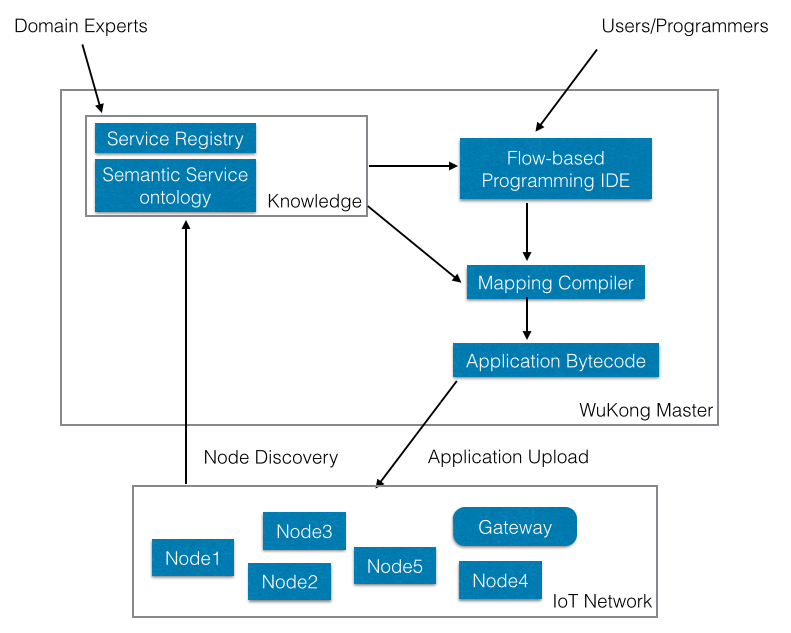
\includegraphics[width=1.0\columnwidth]{five}
\caption{System structure of WuKong}
\label{fig_structure}
\end{figure}


In this section, we proposed WuKong, a service-oriented middleware in IoT. In our study, IoT systems are modeled as distributed system with sensor/actuator/virtual computing components devices that are deployed on different locations in a target environment and connected via RF communication channels. There is a policymaker, called WuKong master, standing on top of the underlying distributed system as figure \ref{fig_structure} shows. WuKong master takes the responsibility for coordinating and monitoring the underlying node devices. To address the challenges to separate virtual application with physical resources, we proposed three functional modules, knowledge base, FBP application IDE, mapping compiler. We elaborate each of them in turns. 

% Master下的knowledge Base
\subsection{Knowledge Base}

The most important part for WuKong master is the comprehensive understanding on top of its underlying distributed system. Master should be able to manage and configure the sensor nodes in a target environment. Based on this purpose, the knowledge of WuKong master consists of two parts, service definition, service registry.  

The definition of standard library of services should be part of the knowledge in WuKong master. The service with commonly-used primitive sensing or actuating or computing capability are defined as atomic service and called WuClass. Light sensor, light actuator, threshold can be examples for atomic services. Similiar to the class definition in object-oriented programming(OOP), we make definition of every atomic services for its functional properties and non-functional properties as figure \ref{fig:atomic} in XML format. Functional properties can be seen as the interface exposed by this service and are waiting to interact with other services. Non-functional properties can express the attributes and characteristics of the service. Non-functional properties will be updated as the IoT system runs. Example definition for atomic service is shown as follows: a temperature service has functional properties such as "readings" and 'refresh rate', non-functional properties such as 'power consumption', 'working range', 'sensitivity', 'precision', 'response time'. 

Compound service is a high-level service component that requires to be composed of several atomic services. In the definition for compound service, master should be aware of all possible substitutional solutions for it[圖2]. Foot step sensor can be seen as a high-level service component. There are several substitude FBP that can achieve the functionality of foot step sensor as defined in figure \ref{fig:compound}. such as and could be realized by either sound-level sensor or PIR sensor or camera sensor. 

% 一些會隨著the running of systems而改變的Property
A node device in IoT system can be equipped with more than one sensors/actuators. The master can generate virtual machine program according to device's capability and characteristics. After uploading it onto the sensor node, this node device can be called "available" to WuKong master because it can respond to master's query and configuration commands. A node device can host multiple services. At the first time to upload virtual machine program, non-functional properties for each residing service will be configureed. Some parameters such as network quality or device quality can vary as IoT system goes. After reasoning and learning process, WuKong master would adjust the parameters for each service on node device. 

\begin{figure}[!t]
\centering
	\begin{minipage}[t]{1.0\linewidth}
        \centering
        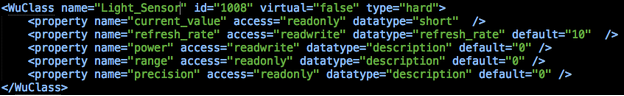
\includegraphics[width=1.0\columnwidth]{six}
        \caption{Example of atomic service definition as master knowledge base}\label{fig:atomic}
    \end{minipage}
    \\[0.2cm]
    \begin{minipage}[t]{1.0\linewidth}
        \centering
        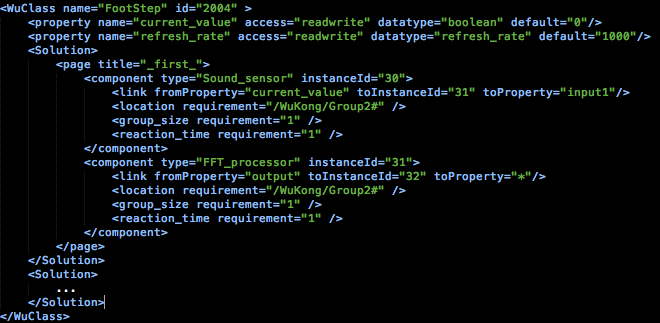
\includegraphics[width=1.0\columnwidth]{seven}
        \caption{Example of compound service definition as master knowledge base}\label{fig:compound}
    \end{minipage}
\end{figure}

\subsection{Flow based Programming IDE}

Most IoT applications are event-driven by nature. When there are some changes in sensors, events are created and passed from one part of IoT system to another. Therefore, the data and control flow should be the programming models for IoT applications as example FBP in figure \ref{fig_service_example}. Using FBP as programming model allow programmers focus on defining the abstract data flow in the application.  

The components that a programmer can use to compose the applications come from a pre-defined component library describe in master knowledge base. Componenets in FBP are defined by their abstract functionalities and interfaces. Each component can be regarded as a virtualized thing since it is possible to match with any physical device as long as the functionality is satisfied. Components can be connected using their exposed interfaces. 

%domain expert 

For each component, programmers can specify requirements so that WuKong master can take it into consideration when mapping. There are two kinds of user requirements described in our system. Point-based requirements are needed to be fulfilled definitely. For example, if the programmer want to get the temperature in living room, the component should be binded with temperature sensors or the device that can give temperature readings. Proximity-based requirements are not required to be fulfill completely but to express the level that the programmer cares for this property. The GUI for setting requirement is shown in figure \ref{requirement}. Programmer can express which properties should considered by selecting the check-box related the specific property. The position of slider is the priority of a property considered by programmer. The value of the slider ranges from 0 to 1. 0 represents that the property should be considered as lowest priority, while 1 stands for the property should be considered at top priority. 

For example, for a light sensor component, if programmer think this light sensor needs to be considered energy efficiency at top priority even if it sacrifices some of its performance, programmer will assign a weight for the power parameter to represent how much he/she cares for power of this component. After specifying point-based requirement and proximity-based requirement, we will do mapping for each service component for its best fit concrete service. 

\begin{figure}[!t]
\centering
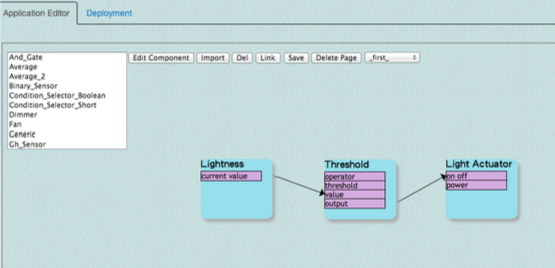
\includegraphics[width=1.0\columnwidth]{fbp}
\caption{The GUI for programming IDE}
\label{fig_sim}
\end{figure}


\begin{figure}[!t]
\centering
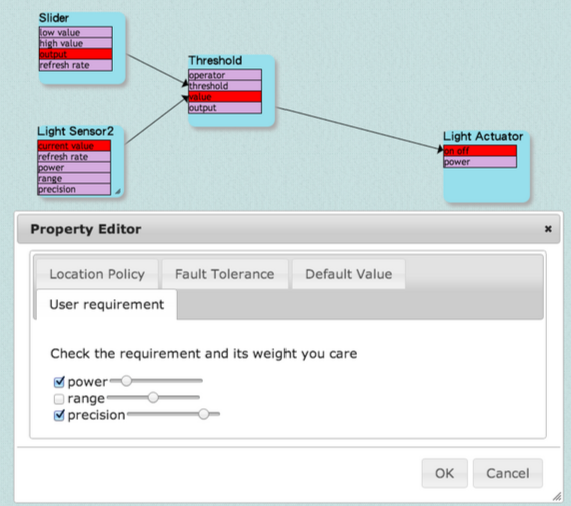
\includegraphics[width=1.0\columnwidth]{fbprequirement}
\caption{The GUI for choose weights}
\label{requirement}
\end{figure}



\subsection{Mapper}

After the programmer finish the application, FBP application IDE will export the application in XML file format. The mapper in WuKong master is to translate the application into hardware programs. After compressing the hardware programs to bytecodes, master then send bytecodes to corresponding node device and finish the application deployment. 

The flow of mapping should go by expansion, matchmaking for sensor/actuator component, matchmaking for computing component. In expansion phase, compound service should be expanded by a sub-FBP and connect to replace the original component. If there are multiple sub-FBP can replace the orignal component, then we should consider many FBPs and choose the best one in the end. 

\begin{figure}[!t]
\centering
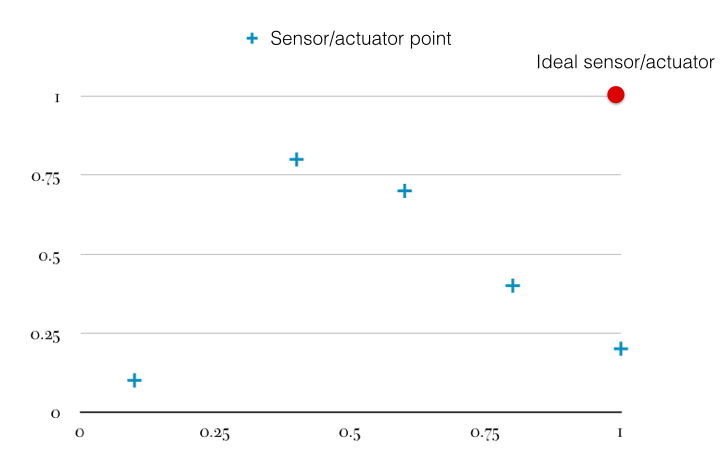
\includegraphics[width=1.0\columnwidth]{coordinate}
\caption{System structure of WuKong}
\label{fig:multidimensional}
\end{figure}

After expansion, we then perform one-to-one sensor/actuator matchmaking for each component. Matchmaking is a process that WuKong master decides the relationship between component and physical resource. Here we propose an user-oriented mapping scheme. Given the requirments provided by programmers, WuKong master will first filter all services from service repository by point-based requirement(e.g type, location). For the filtered result, we plot each candidate sensor/actuator on multi-dimensional space where each dimension is regarded as an attribute. As figure \ref{fig:multidimensional} shows. 
An ideal sensor $U$ in the multidimensional space represents highest value for all attributes as the desired point shown in the figure. Then, among the filtered services on the figure, master will choose the most suitable resource by evaluating matching score. For a service $S^\alpha$, the matching score is defined as the distance to the ideal sensor $U$ on multi-dimensional space, 

$Score(S^\alpha, U) = \sqrt{ \frac{\sum\limits_{i=0}^n(W_i(U_i - S_i^\alpha)^2)}{\sum\limits_{i=0}^n(W_i)}}$


$AvrScore(FBP) = \frac{\sum\limits_{j=0}^n \text{argmin } score(S_j^\alpha, U_j)}{\sum\limits_{j=0}^n(C_j)}$
The nearest sensor/actuator will be chosen to bind with the component.
\begin{algorithm}[h]
    \caption{The execution flow of mapping}
    \begin{algorithmic}[1]
        \REQUIRE $S$ is the set of all sensors/actuators, $P$ is the set of user requirements;
        \ENSURE The most matching sensor/actuator with lowest matching score according to user requirements. 
        \STATE $S_{\text{filtered}} \leftarrow \text{Filtering}(S)$
        \STATE $P$ is the set of user requirements  
          
    \end{algorithmic}
\end{algorithm}

% You must have at least 2 linexs in the paragraph with the drop letter
% (should never be an issue)

% \subsection{Subsection Heading Here}
% Subsection text here.


% \subsubsection{Subsubsection Heading Here}
% Subsubsection text here.

% \section{Type style and Fonts}
% Wherever Times is specified, Times Roman or Times New Roman may be used. If neither is available on your system, please use the font closest in appearance to Times. Avoid using bit-mapped fonts if possible. True-Type 1 or Open Type fonts are preferred. Please embed symbol fonts, as well, for math, etc.


% An example of a floating figure using the graphicx package.
% Note that \label must occur AFTER (or within) \caption.
% For figures, \caption should occur after the \includegraphics.
% Note that IEEEtran v1.7 and later has special internal code that
% is designed to preserve the operation of \label within \caption
% even when the captionsoff option is in effect. However, because
% of issues like this, it may be the safest practice to put all your
% \label just after \caption rather than within \caption{}.
%
% Reminder: the "draftcls" or "draftclsnofoot", not "draft", class
% option should be used if it is desired that the figures are to be
% displayed while in draft mode.
%
%\begin{figure}[!t]
%\centering
%\includegraphics[width=2.5in]{myfigure}
% where an .eps filename suffix will be assumed under latex, 
% and a .pdf suffix will be assumed for pdflatex; or what has been declared
% via \DeclareGraphicsExtensions.
%\caption{Simulation Results}
%\label{fig_sim}
%\end{figure}

% Note that IEEE typically puts floats only at the top, even when this
% results in a large percentage of a column being occupied by floats.


% An example of a double column floating figure using two subfigures.
% (The subfig.sty package must be loaded for this to work.)
% The subfigure \label commands are set within each subfloat command, the
% \label for the overall figure must come after \caption.
% \hfil must be used as a separator to get equal spacing.
% The subfigure.sty package works much the same way, except \subfigure is
% used instead of \subfloat.
%
%\begin{figure*}[!t]
%\centerline{\subfloat[Case I]\includegraphics[width=2.5in]{subfigcase1}%
%\label{fig_first_case}}
%\hfil
%\subfloat[Case II]{\includegraphics[width=2.5in]{subfigcase2}%
%\label{fig_second_case}}}
%\caption{Simulation results}
%\label{fig_sim}
%\end{figure*}
%
% Note that often IEEE papers with subfigures do not employ subfigure
% captions (using the optional argument to \subfloat), but instead will
% reference/describe all of them (a), (b), etc., within the main caption.


% An example of a floating table. Note that, for IEEE style tables, the 
% \caption command should come BEFORE the table. Table text will default to
% \footnotesize as IEEE normally uses this smaller font for tables.
% The \label must come after \caption as always.
%
%\begin{table}[!t]
%% increase table row spacing, adjust to taste
%\renewcommand{\arraystretch}{1.3}
% if using array.sty, it might be a good idea to tweak the value of
% \extrarowheight as needed to properly center the text within the cells
%\caption{An Example of a Table}
%\label{table_example}
%\centering
%% Some packages, such as MDW tools, offer better commands for making tables
%% than the plain LaTeX2e tabular which is used here.
%\begin{tabular}{|c||c|}
%\hline
%One & Two\\
%\hline
%Three & Four\\
%\hline
%\end{tabular}
%\end{table}


% Note that IEEE does not put floats in the very first column - or typically
% anywhere on the first page for that matter. Also, in-text middle ("here")
% positioning is not used. Most IEEE journals/conferences use top floats
% exclusively. Note that, LaTeX2e, unlike IEEE journals/conferences, places
% footnotes above bottom floats. This can be corrected via the \fnbelowfloat
% command of the stfloats package.

\section{Conclusion}
% conference papers do not normally have an appendix

As the number of IoT devices grows, it becomes challenging to deploy applications through the network. To make programming on IoT simple is a must, since in the future everyone should be able to interact with IoT network. Make their request throught an user-friendly tool. High-level master knowledge is needed, since IoT middleware should intelligently help programmer to find out their solution to requested IoT application. We can raise the level of programming abstraction. We proposed a service-oriented middleware to suppport programmer to easier deploy their IoT application. In the future, we will further research on semantic matchmaking suppport in IoT middleware. With the aim to support more non-WSN expert to interact with the world of IoT.  
% use section* for acknowledgement
\section*{Acknowledgment}
This work was also supported by National Science Council, National Taiwan University and Intel Corporation under Grants NSC102-2911-I-002-001 and NTU103R7501.

% trigger a \newpage just before the given reference
% number - used to balance the columns on the last page
% adjust value as needed - may need to be readjusted if
% the document is modified later
%\IEEEtriggeratref{8}
% The "triggered" command can be changed if desired:
%\IEEEtriggercmd{\enlargethispage{-5in}}

% references section

% can use a bibliography generated by BibTeX as a .bbl file
% BibTeX documentation can be easily obtained at:
% http://www.ctan.org/tex-archive/biblio/bibtex/contrib/doc/
% The IEEEtran BibTeX style support page is at:
% http://www.michaelshell.org/tex/ieeetran/bibtex/
%\bibliographystyle{IEEEtran}
% argument is your BibTeX string definitions and bibliography database(s)
%\bibliography{IEEEabrv,../bib/paper}
%
% <OR> manually copy in the resultant .bbl file
% set second argument of \begin to the number of references
% (used to reserve space for the reference number labels box)
% \begin{thebibliography}{1}

% \bibitem{IEEEhowto:kopka}
% H.~Kopka and P.~W. Daly, \emph{A Guide to \LaTeX}, 3rd~ed.\hskip 1em plus
%   0.5em minus 0.4em\relax Harlow, England: Addison-Wesley, 1999.
\bibliographystyle{IEEEtran}
\bibliography{thesis}

% \end{thebibliography}




% that's all folks
\end{document}


